% ---------------------------------------------------------------------------
\FloatBarrier
\section{Reproduction of the Paper's Models (RQ1)}
\label{sec:reproduction}

Before comparing new models, we rebuilt the three models of
Severson~\textit{et al.}~\cite{severson2019} on our cleaned data. If our
pipeline reproduces their Table~1, any later difference between models can be
trusted to come from the models, not from the data handling. The code is in
\texttt{src/features.py}, \texttt{src/reproduce.py} and
\texttt{src/evaluate.py}; the notebook \texttt{notebooks/02\_reproduction.ipynb}
re-runs every step shown in this section.

\subsection{Task}
The input is the data of the first 100 cycles of a cell. The output is its
cycle life, the first cycle at which the discharge capacity falls below
0.88\,Ah. Models are fitted to $\log_{10}$(cycle life): lives span
148--2237 cycles, and on the log scale a 10\,\% error weighs the same for
a short- and a long-lived cell. All fitting and tuning uses the 41 training
cells only. The 43 primary-test cells come from the same two batches as the
training cells; the 40 secondary-test cells come from the 2018-04-12 batch,
run about a year later with a different procedure (Table~\ref{tab:batches}).

\subsection{The $\dq$ signal}
\texttt{Qdlin} is the discharge capacity as a function of voltage during the
\Crate{4} constant-current discharge, interpolated by the authors on a
1000-point grid from 3.5 to 2.0\,V. The paper's main feature is the change
in this curve between cycles 10 and 100,
\begin{equation}
  \dq = Q_{100}(V) - Q_{10}(V).
\end{equation}
Fig.~\ref{fig:p2dq} shows why it is useful. For the longest- and
shortest-lived training cells (2160 and 300 cycles), the discharge curves at
cycle 100 differ only a little from those at cycle 10
(Fig.~\ref{fig:p2dq}a), but $\dq$ differs by an order of magnitude
(Fig.~\ref{fig:p2dq}b): its minimum is $-11$\,mAh for the long-lived cell and
$-135$\,mAh for the short-lived one. Over all training cells, $\dq$ grows
steadily deeper as life gets shorter (Fig.~\ref{fig:p2dq}d). The capacity
itself (Fig.~\ref{fig:p2dq}c) is a weaker early signal: most of the fade
comes after cycle 100. The paper attributes the early change in curve shape
to loss of active material at the negative electrode, which alters the
voltage curve before it reduces capacity~\cite{severson2019}.

\begin{figure*}[t]
  \centering
  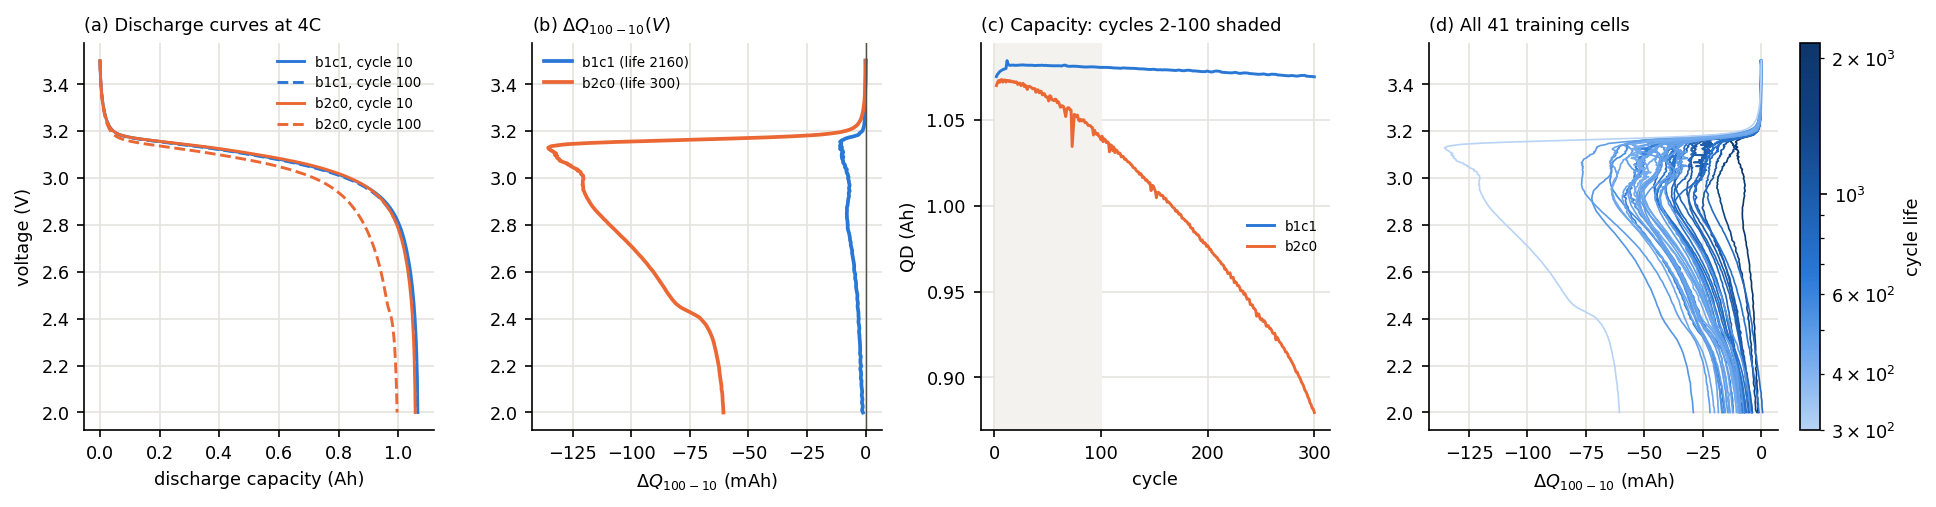
\includegraphics[width=\textwidth]{fig_p2_dq}
  \caption{The $\dq$ feature. (a) Discharge curves at cycles 10 and 100 of
  the longest-lived (\texttt{b1c1}) and shortest-lived (\texttt{b2c0})
  training cells. (b) Their $\dq$. (c) Their capacity; features use only
  the shaded cycles 2--100. (d) $\dq$ of all 41 training cells, coloured by
  cycle life (cf.\ Fig.~2a of~\cite{severson2019}).}
  \label{fig:p2dq}
\end{figure*}

\subsection{Candidate features}
Table~\ref{tab:features} lists the 20 candidate features of the paper's
Supplementary Table~1, all computed from cycles $\le 100$, and marks the
subsets used by the three models. The $\dq$ curve is reduced to summary
statistics across the 1000 voltage points; the other features describe the
capacity fade, the charging policy (through the charge time), the cell
temperature and the internal resistance (IR). Where the paper's
Supplementary Note~1 is ambiguous, we made the choices in
Table~\ref{tab:implchoices}. As a check, the features of one cell were
recomputed by hand in the notebook and agree with \texttt{src/features.py}
to machine precision.

\begin{table*}[t]
\centering
\caption{The 20 candidate features of~\cite{severson2019} (Supplementary
Table~1), computed from cycles $\le 100$, and the subsets used by the
variance (V), discharge (D) and full (F) models. $r$: Pearson correlation
with $\log_{10}$(cycle life) over the 41 training cells.}
\label{tab:features}
\small
\setlength{\tabcolsep}{4pt}
\begin{tabular}{@{}llp{0.34\textwidth}cccr@{}}
\toprule
Group & Feature & Definition & V & D & F & $r$ \\
\midrule
\multirow{6}{*}{$\dq$}
 & \texttt{dq\_log\_var}  & $\log_{10}$ variance (sample, $p-1$) & \checkmark & \checkmark & \checkmark & $-0.90$ \\
 & \texttt{dq\_log\_min}  & $\log_{10}|\min|$ & & \checkmark & \checkmark & $-0.89$ \\
 & \texttt{dq\_log\_mean} & $\log_{10}|\mathrm{mean}|$ & & & & $-0.88$ \\
 & \texttt{dq\_log\_skew} & $\log_{10}|$skewness$|$ & & \checkmark & & $+0.38$ \\
 & \texttt{dq\_log\_kurt} & $\log_{10}$ kurtosis & & \checkmark & & $+0.20$ \\
 & \texttt{dq\_log\_2v}   & $\log_{10}|\Delta Q(2.0\,\mathrm{V})|$ & & & & $-0.72$ \\
\midrule
\multirow{7}{*}{Capacity}
 & \texttt{qd\_slope\_2\_100}, \texttt{qd\_icpt\_2\_100} & slope, intercept of a line fitted to QD over cycles 2--100 & & & \checkmark & $+0.40$, $+0.28$ \\
 & \texttt{qd\_slope\_91\_100}, \texttt{qd\_icpt\_91\_100} & the same over cycles 91--100 & & & & $+0.46$, $+0.03$ \\
 & \texttt{qd\_2} & QD at cycle 2 & & \checkmark & \checkmark & $+0.33$ \\
 & \texttt{qd\_max\_minus\_2} & max QD $-$ QD at cycle 2 & & \checkmark & & $+0.15$ \\
 & \texttt{qd\_100} & QD at cycle 100 & & & & $+0.47$ \\
\midrule
\multirow{7}{*}{Other}
 & \texttt{chargetime\_avg\_2\_6} & mean charge time, cycles 2--6 & & & \checkmark & $+0.77$ \\
 & \texttt{temp\_integral\_2\_100} & $\int T\,dt$ summed over cycles 2--100 & & & \checkmark & $-0.72$ \\
 & \texttt{temp\_max\_2\_100}, \texttt{temp\_min\_2\_100} & max, min can temperature & & & & $-0.34$, $+0.30$ \\
 & \texttt{ir\_min\_2\_100} & minimum IR, cycles 2--100 & & & \checkmark & $-0.39$ \\
 & \texttt{ir\_100\_minus\_2} & IR(100) $-$ IR(2) & & & \checkmark & $+0.38$ \\
 & \texttt{ir\_2} & IR at cycle 2 & & & & $-0.57$ \\
\bottomrule
\end{tabular}
\end{table*}

\begin{table}[t]
\centering
\caption{Implementation choices where the paper's Supplementary Note~1 is
ambiguous.}
\label{tab:implchoices}
\setlength{\tabcolsep}{3pt}
\begin{tabular}{@{}p{0.30\columnwidth}p{0.64\columnwidth}@{}}
\toprule
Item & Choice \\
\midrule
Variance & sample variance ($p-1$), as in Note~1 \\
Skewness, kurtosis & standard moment ratios $m_3/m_2^{1.5}$, $m_4/m_2^2$; the
Note~1 skewness denominator is read as a typo \\
Capacity features & \texttt{QD\_clean} (glitch cycles removed, rule B3) \\
Single-cycle values & nearest cycle with a finite value within $\pm3$ \\
Temperature integral & sum over cycles of the trapezoidal $\int T\,dt$ of the
raw traces, leaving out sample gaps $>10$\,min (rule B10) \\
Missing values & training-set median (only \texttt{b1c18}'s IR, rule B9) \\
\bottomrule
\end{tabular}
\end{table}

\textbf{Correlation with life.} Fig.~\ref{fig:p2corr} and the last column
of Table~\ref{tab:features} show how strongly each feature relates to life
on the training cells. The three $\dq$ location and spread statistics are
the strongest ($|r| = 0.88$--$0.90$). The next two are partly
\emph{batch} effects, because the 41 training cells come from two batches
that differ both in procedure and in life (\texttt{b1}: mean 889 cycles;
\texttt{b2}: 469). The charge time ($r = +0.77$) identifies the charging
policy: within \texttt{b1}, whose policies take 9.0--13.4\,min, longer
charge times (lower currents) give longer lives ($r = +0.77$), while all
\texttt{b2} policies take about 10.2\,min. The temperature integral
($r=-0.72$) mostly measures cycle duration. \texttt{b2} cycles include two
5-min rests, so they are longer and accumulate a larger integral (191{,}500
vs.\ 166{,}900\,\textdegree C$\cdot$min on average). Within a batch its
correlation with life is weak ($r=-0.14$ in \texttt{b1}, $+0.45$ in
\texttt{b2}). The capacity features are weak ($|r| \le 0.47$), which
confirms that capacity alone is a poor early predictor.

\begin{figure}[t]
  \centering
  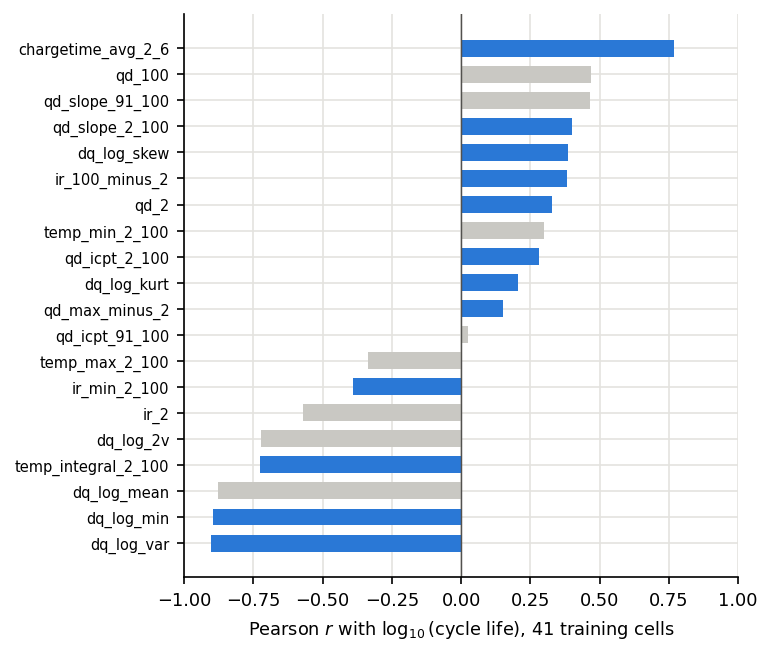
\includegraphics[width=0.9\columnwidth]{fig_p2_corr}
  \caption{Pearson correlation of each candidate feature with
  $\log_{10}$(cycle life) over the 41 training cells. Blue: used by the
  discharge or full model.}
  \label{fig:p2corr}
\end{figure}

\subsection{Models}
All three models predict $\log_{10}$(cycle life); predictions are converted
back to cycles before scoring. Each is a pipeline of three steps:
\begin{enumerate}
  \item \textbf{Imputation} of missing values with the training-set median.
  Only \texttt{b1c18}'s IR features are missing (rule B9).
  \item \textbf{Standardisation} of each feature to zero mean and unit
  variance (on the training cells). This puts the features on one scale,
  so the penalty below treats them equally and the coefficients can be
  compared.
  \item \textbf{Regression.}
  \begin{itemize}
    \item \emph{Variance model}: ordinary least squares on one feature, with
    no tuning, as in the paper. The fit is
    $\log_{10}(\text{life}) = 1.346 - 0.396\,\log_{10}\mathrm{Var}(\dq)$.
    \item \emph{Discharge and full models}: the elastic net, as in the
    paper. It minimises
    \begin{equation}
      \frac{1}{2n}\lVert \mathbf{y}-X\mathbf{w}\rVert_2^2
      + \alpha\,\rho\,\lVert\mathbf{w}\rVert_1
      + \frac{\alpha(1-\rho)}{2}\lVert\mathbf{w}\rVert_2^2 ,
    \end{equation}
    where $\alpha$ sets the penalty strength and $\rho$ (the $\ell_1$
    ratio) the mix of the two penalties. The $\ell_1$ term can set
    weights exactly to zero, which selects features; the $\ell_2$ term
    shares weight among correlated features. With only 41 training cells,
    the penalty keeps the model from overfitting.
  \end{itemize}
\end{enumerate}
$\alpha$ (100 values) and $\rho$ (8 values between 0.1 and 1) are chosen by
4-fold cross-validation repeated 10 times on the training cells (the paper
uses 4-fold cross-validation with Monte Carlo sampling).
Fig.~\ref{fig:p2cv} shows the cross-validation error. A small $\alpha$
gives the unpenalised least-squares fit; beyond $\alpha \approx 0.01$--$0.1$
(depending on $\rho$) the error rises steeply as the penalty removes real
signal. Both models choose
$\rho = 0.1$, close to ridge regression, with $\alpha = 0.022$ (discharge,
6 of 6 features kept) and $\alpha = 0.039$ (full, 7 of 9 kept). The full
model leaves out the four cells whose temperature probe lost contact (rule
B6), as the paper does. The test sets are evaluated once. RMSE and mean
percentage error are computed on cycles, not on the log scale.

\begin{figure}[t]
  \centering
  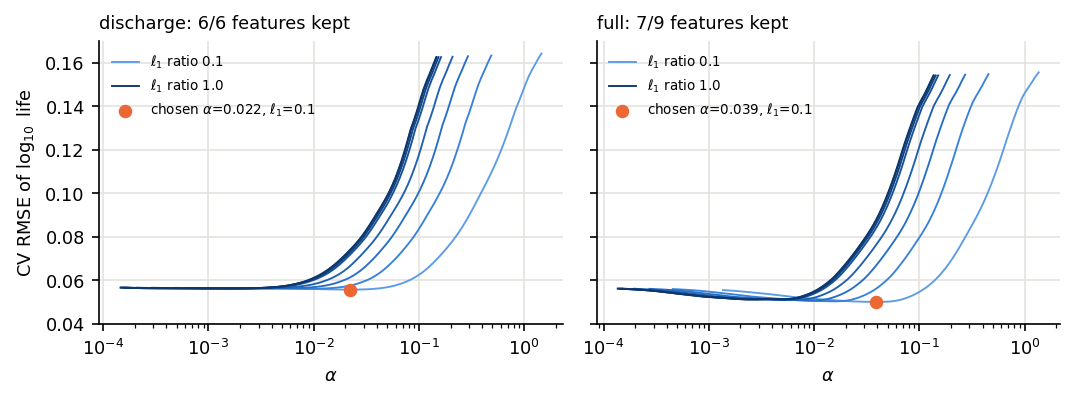
\includegraphics[width=\columnwidth]{fig_p2_cv}
  \caption{Cross-validation RMSE of $\log_{10}$(life) against the penalty
  strength $\alpha$, one line per $\ell_1$ ratio. The dot marks the chosen
  setting.}
  \label{fig:p2cv}
\end{figure}

\textbf{Baselines.} The \emph{constant} baseline predicts the training mean
of $\log_{10}$(life) for every cell, i.e.\ the geometric mean of the
training lives; this reproduces the paper's Supplementary Table~3 exactly,
whereas the arithmetic mean does not. The \emph{policy-mean} baseline (our
addition) predicts the geometric-mean training life of cells with the same
charging policy, and the constant for unseen policies.

\subsection{Results}
Table~\ref{tab:repro} compares our errors with the paper's. The
\textbf{variance model matches to within one cycle} on every split. Since
this model has no tuning, the match tests only the data, the $\dq$ feature,
the labels and the split, and confirms that all four are identical to the
paper's. The discharge model is within 1--9\,\% of the paper's RMSE. The
full model is close on the test sets (primary 125 vs.\ 118 cycles,
secondary 220 vs.\ 214) and less close on training (67 vs.\ 51). The
ranking of the three models is the same as in the paper on every split,
including the paper's counter-intuitive result that the full model is
\emph{worse} than the discharge model on the secondary test set. The paper
attributes this to the secondary batch's extra year of calendar ageing,
which lowers its initial capacity and biases the capacity features.

\begin{table*}[t]
\centering
\caption{Reproduction of the paper's Table~1 and the constant baseline of
its Supplementary Table~3. Each entry is RMSE (cycles) / mean percentage
error; paper values in parentheses. ``Primary excl.'' leaves out the anomalous
cell \texttt{b2c1}. The policy-mean baseline is ours.}
\label{tab:repro}
\begin{tabular}{@{}lcccc@{}}
\toprule
Model & Train & Primary test & Primary excl. & Secondary test \\
\midrule
Constant      & 327 / 29.6\,\% (327 / 29.6) & 401 / 35.0\,\% (401 / 34.9) & 399 / 28.2\,\% (399 / 28.2) & 511 / 36.1\,\% (511 / 36.1) \\
Policy mean   & 46 / 1.6\,\%  & 173 / 27.3\,\% & 159 / 20.3\,\% & 509 / 36.0\,\% \\
Variance      & 104 / 14.1\,\% (103 / 14.1) & 138 / 14.7\,\% (138 / 14.7) & 138 / 13.2\,\% (138 / 13.2) & 196 / 11.4\,\% (196 / 11.4) \\
Discharge     & 69 / 9.2\,\% (76 / 9.8)     & 90 / 12.6\,\% (91 / 13.0)   & 85 / 9.4\,\% (86 / 10.1)    & 167 / 9.9\,\% (173 / 8.6) \\
Full          & 67 / 6.8\,\% (51 / 5.6)     & 125 / 11.0\,\% (118 / 14.1) & 122 / 8.0\,\% (100 / 7.5)   & 220 / 11.2\,\% (214 / 10.7) \\
\bottomrule
\end{tabular}
\end{table*}

\begin{figure*}[t]
  \centering
  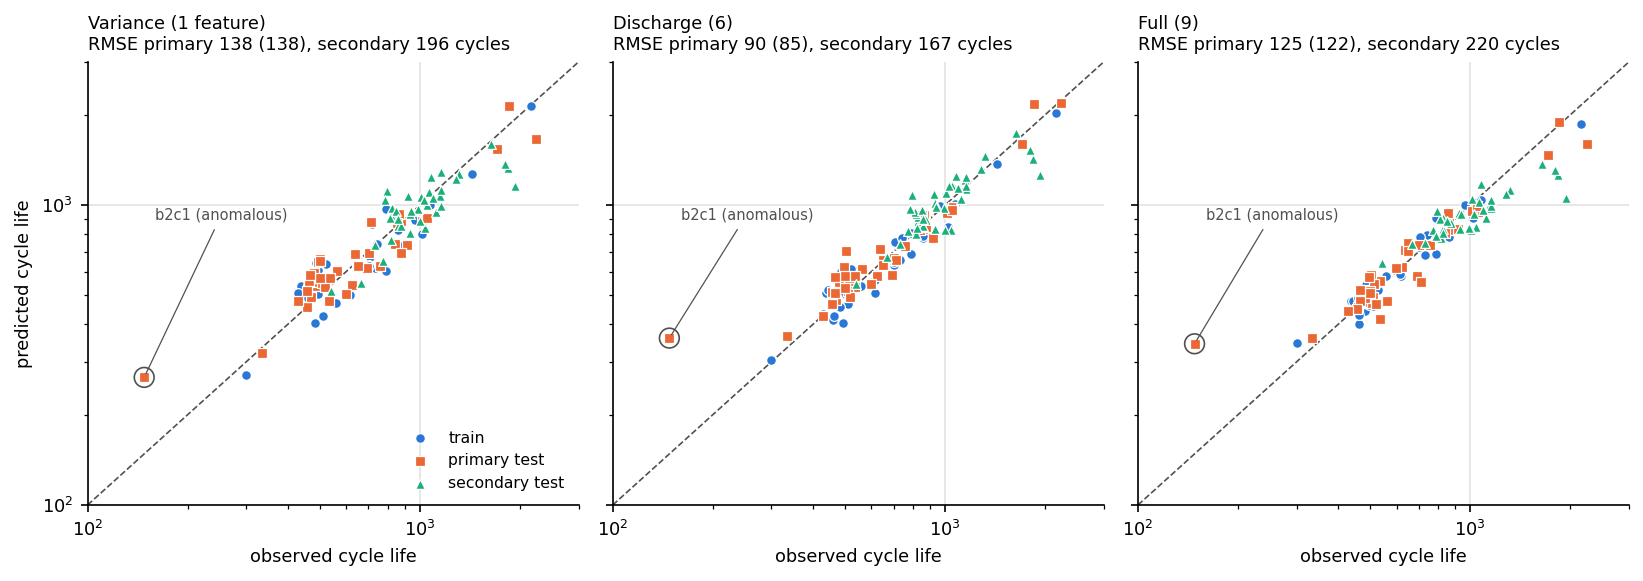
\includegraphics[width=\textwidth]{fig_p2_parity}
  \caption{Predicted vs.\ observed cycle life for the three reproduced models
  (log axes; cf.\ the paper's Fig.~3). Dashed line: perfect prediction.
  RMSE in parentheses excludes the anomalous cell \texttt{b2c1} (circled). In
  all three models, the longest-lived secondary-test cells are under-predicted.}
  \label{fig:parity}
\end{figure*}

\textbf{Coefficients.} The paper prints the full model's coefficients on
standardised features (its Supplementary Fig.~5). Ours have the same sign for
all nine features and similar magnitudes (Table~\ref{tab:coef}). A
coefficient of $-0.049$ on $\log_{10}\mathrm{Var}(\dq)$ means that one
standard deviation more of this feature lowers $\log_{10}$(life) by 0.049,
i.e.\ shortens life by about 11\,\%. Like the paper, our elastic net gives
the fade-curve intercept a weight of essentially zero. It also zeroes the
fade-curve slope, to which the paper gives a small weight.

\begin{table}[t]
\centering
\caption{Full-model coefficients on standardised features (target
$\log_{10}$ life): ours vs.\ the paper's Supplementary Fig.~5.}
\label{tab:coef}
\begin{tabular}{@{}lrr@{}}
\toprule
Feature & Ours & Paper \\
\midrule
$\log_{10}\mathrm{Var}(\dq)$ & $-0.049$ & $-0.071$ \\
$\log_{10}|\min\dq|$ & $-0.040$ & $-0.029$ \\
Charge time, cycles 2--6 & $+0.033$ & $+0.039$ \\
Temperature integral & $-0.029$ & $-0.036$ \\
Capacity, cycle 2 & $+0.025$ & $+0.022$ \\
Minimum IR & $-0.021$ & $-0.007$ \\
IR(100)$-$IR(2) & $-0.000$ & $-0.013$ \\
Fade slope, cycles 2--100 & $0.000$ & $-0.013$ \\
Fade intercept, cycles 2--100 & $0.000$ & $0.000$ \\
\bottomrule
\end{tabular}
\end{table}

\textbf{Stability.} Repeating the cross-validation with ten different random
seeds changes the test RMSE by only a few cycles (discharge: primary 89--91,
secondary 167--170; full: primary 117--128, secondary 218--222). The
remaining differences from the paper are of the same size as this spread.
They are expected given the paper's different software (MATLAB), its own
random sampling, and its spline fit of the discharge curves.

\textbf{Where the errors come from.} The errors are concentrated in a few
cells. \texttt{b1c2}, the longest-lived cell in the dataset (2237 cycles), is
predicted at 1594 cycles by the full model. It accounts for 63\,\% of that
model's squared error on the primary set, and 67\,\% once \texttt{b2c1} is
excluded; without it, the primary RMSE excluding \texttt{b2c1} would be 71
instead of 122 cycles. More generally, the longest-lived cells are
under-predicted by all three models (Fig.~\ref{fig:parity}): few training
cells live beyond 1500 cycles, so the fitted line is poorly constrained
there. At the other end, the anomalous cell \texttt{b2c1} (148 cycles) is
predicted at 266--360 cycles by the three models; its early failure is not
visible in the first 100 cycles.

\subsection{A data fault found by the reproduction}
The first full-model fit predicted 0 cycles for \texttt{b1c18} (observed
life 691; primary RMSE 162 instead of 125 after the fix). The cause was a fault in
this cell's records for cycles 2--53 (Fig.~\ref{fig:p2b1c18}). The IR logger
was stuck, repeating 19.886\,m$\Omega$ for 52 cycles; no other cell repeats
a value more than twice. And every record contains a corrupt time stamp that
jumps by 35--67\,h, which inflates the temperature integral. Measured
against the training cells, the unfiltered integral lies 372 standard
deviations above the mean, and $\mathrm{IR}(100)-\mathrm{IR}(2)$ lies 11.9
below it. A linear model extrapolates such values to a life of zero. Rules
B9 and B10 (Table~\ref{tab:cleaning}) fix both; the prediction for
\texttt{b1c18} becomes 578 cycles. The paper's numbers thus served as a
check that exposed a fault the earlier cleaning had missed, which is why
the reproduction was done before any new model.

\begin{figure}[t]
  \centering
  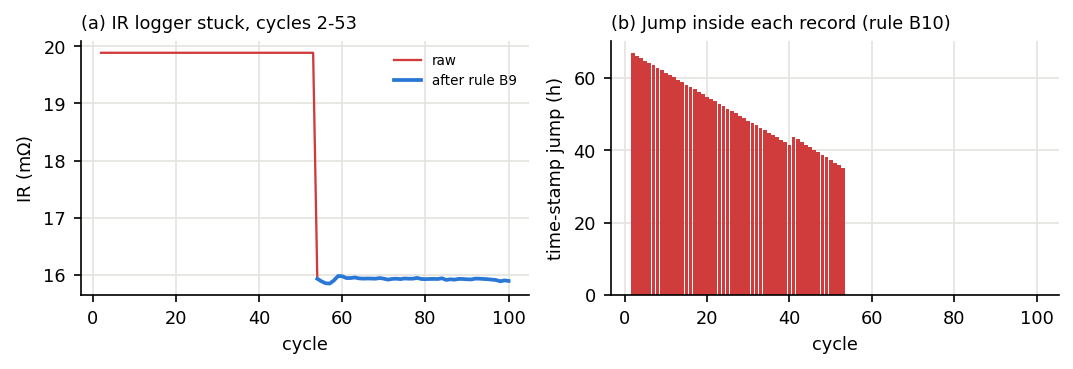
\includegraphics[width=\columnwidth]{fig_p2_b1c18}
  \caption{The data fault in \texttt{b1c18}. (a) IR stuck at one value for
  cycles 2--53, set to missing by rule B9. (b) Length of the time-stamp
  jump inside each cycle record, left out of the temperature integral by
  rule B10.}
  \label{fig:p2b1c18}
\end{figure}

\textbf{Baselines.} The policy-mean baseline does better than the constant
on the primary set (173 vs.\ 401 cycles), since the primary cells share
charging policies with training. But it has nothing to offer on the
secondary set, whose policies never appear in training, and it is still
clearly worse than the single-feature variance model. Both baselines confirm
that the $\dq$ features carry the predictive information.

\textbf{Answer to RQ1.} Yes: the paper's results are reproduced, exactly for
the variance model and to within the cross-validation spread for the others,
with the same model ranking and the same coefficient signs. The pipeline
(features, models and evaluation) is therefore a sound base for the model
comparison, and the errors in Table~\ref{tab:repro} are the baselines that
new models and the physics-informed features (F4) have to beat.
